% This must be in the first 5 lines to tell arXiv to use pdfLaTeX, which is strongly recommended.
\pdfoutput=1
% In particular, the hyperref package requires pdfLaTeX in order to break URLs across lines.


\documentclass[11pt]{article}

% Remove the "review" option to generate the final version.
\usepackage[review]{ACL2023}
%\usepackage[anonymous]{ACL2023}

% Standard package includes
\usepackage{times}
\usepackage{latexsym}
\usepackage{graphicx} 

% For proper rendering and hyphenation of words containing Latin characters (including in bib files)
\usepackage[T1]{fontenc}
% For Vietnamese characters
% \usepackage[T5]{fontenc}
% See https://www.latex-project.org/help/documentation/encguide.pdf for other character sets

% This assumes your files are encoded as UTF8
\usepackage[utf8]{inputenc}

% This is not strictly necessary, and may be commented out.
% However, it will improve the layout of the manuscript,
% and will typically save some space.
\usepackage{microtype}

% This is also not strictly necessary, and may be commented out.
% However, it will improve the aesthetics of text in
% the typewriter font.
\usepackage{inconsolata}
\usepackage{multirow}

% If the title and author information does not fit in the area allocated, uncomment the following
%
\setlength\titlebox{5cm}

%
% and set <dim> to something 5cm or larger.
\begin{document}

\title{COMP550 Project Report: Comparative Analysis of Chinese Word Segmentation in Sentiment Analysis and Text Classification\thanks{ChatGPT was used for correcting grammatical errors and refining this report. No content is AI generated.}}
\author{Zihan Wang \\
  %Department of Electrical Engineering\\
  McGill University\\
  \texttt{zihan.wang5@mail.mcgill.ca} \\
  \And
  Jack Wei \\
  %Department of Electrical Engineering\\
  McGill University\\
  \texttt{yi.wei4@mail.mcgill.ca} \\
  \And
  Xijuan Sun \\
  %Department of Electrical Engineering\\
  McGill University\\
  \texttt{xijuan.sun@mail.mcgill.ca} \\
  }

\maketitle

\begin{abstract}
This project explores the complexity of Chinese text analysis, evaluating the efficacy of different tokenization approaches (character, word, pinyin) and the inclusion of bigrams at the character level in text classification and sentiment analysis. This study also examines the effect of stopwords removal and how the pre-trained word2vec embeddings enhance models' performance measured by accuracy and F1 score. Logistic Regression (LR) and Long Short-Term Memory (LSTM) networks, along with their variants, are tested on the \textit{onlineshopping10cats} dataset. Our results indicate that for LSTM models with distributed representation, word-level and character-level tokenization offer comparable performance in sentiment analysis and text classification. Conversely, logistic regression models utilizing bag-of-words features perform best with lower-granularity tokens like words and character bigrams.
\end{abstract}

\section{Introduction}
Chinese Natural Language Processing (NLP) tasks present distinct challenges, primarily due to the absence of explicit word boundaries inherent to the language. This absence renders word segmentation a critical and complex task. In this investigation, we probe into various approaches of Chinese text tokenization. Character-level tokenization is a straightforward method which does not need extensive linguistic knowledge but may miss semantic meanings of compound words. In contrast, word-level tokenization aligns more naturally with Chinese linguistic patterns; however, it contends with the challenge of ambiguous word boundaries. To tackle this complexity, several tools such as \textit{HanLP}, \textit{THULAC}, \textit{SnowNLP}, and \textit{Jieba} have been developed, each designed to adeptly deal with the uniqueness of the Chinese language, such as its abundance of homophones. 

Sub-character tokenization schemes, particularly those utilizing phonetic representations like pinyin, offer an alternative approach. As introduced by~\citep{si-etal-2023-sub}, these schemes not only increase computational efficiency by reducing input dimension of the embedding layer but also are robust to homophone typos by embedding them to the same vector representation. However, a potential drawback of the pinyin-level tokenization scheme is their tendency to neglect the semantic context because of their emphasis on phonetics. This study aims to assess the impact of these tokenization methods on the performance of NLP models in Chinese text analysis tasks.
 
Beyond tokenization, word2vec \citep{mikolov2013efficient} embedding plays a crucial role in analyzing Chinese context. It transforms words or characters into vectors that encapsulate semantic patterns, allowing models to discern linguistic contexts and relationships. In Chinese NLP, the ability of word2vec to capture linguistic regularities and semantic relationships in a dense vector space significantly enhances tasks like similarity detection and sentiment analysis~\citep{li2018ana}. 

Our work applies different models to evaluate the influence of different tokenization strategies on two common NLP tasks: sentiment analysis and text classification. Sentiment analysis is integral for extracting the emotional tone from text, which is vital for understanding consumer behavior in online reviews. Text classification, on the other hand, is essential for systematically categorizing text, crucial for effective information retrieval. Given the importance of contextual understanding in Chinese, models capable of capturing long-term dependencies, such as LSTM, are particularly useful for these tasks.

In this project, Logistic Regression (LR) and LSTM models are employed for exploring the impact of various tokenization schemes, including character-level, word-level, and pinyin-level, along with the exploration of bigrams in character-level tokenization for text classification and sentiment analysis tasks. Moreover, the word2vec embedding is also introduced to LSTMs to evaluate its ability in capturing linguistic regularities. Taking into account of these confounding factors in model selection, the primary objective of this study is to determine the optimal level of token granularity for sentiment analysis and text classification based on model performance as measured by accuracy and F1 score. Experiments are conducted on the \textit{onlineshopping10cats} dataset, which is widely used in Chinese text analysis~\citep{sun2022word, graves2005}.

The contributions of this work are as follows: i. Systematically explored the effect of various Chinese tokenization methods for linear and neural models in sentiment analysis and text classification tasks ii. Explored the effectiveness of word2vec embeddings for both character and word tokens in Chinese text analysis. iii. Investigated the performance of tone-less pinyin tokenization for sentiment analysis and text classification tasks.

\section{Related Work}
The segmentation of Chinese text has been extensively researched due to the language's absence of explicit word boundaries. The study~\citep{xue-2003-chinese} have pointed out that the character-level tokenization might not fully capture the semantic meaning of phrases, as individual Chinese characters often convey less distinct information than full words. \citep{zhou-2003-chunking} discussed how word-level tokenization, which aligns more closely with nature of Chinese, could enhance semantic understanding of models in Chinese NLP tasks. Recent studies, such as~\citep{sun2022word}, employ the word-level tokenization tool \textit{Jieba}, which leverages dictionary-based methods and Hidden Markov Models to improve segmentation efficiency. Moreover, the research~\citep{si-etal-2023-sub} has shown that the phonetic-based approach of pinyin-level tokenization can address homophony and improve computational efficiency, but may sacrifice semantic depth due to its focus on pronunciation. In this study, we investigated the impact of three distinct tokenization schemes, as well as the application of bigrams feature extraction in character-level tokenization, for sentiment analysis and text classification tasks. To the best of our knowledge, this is the first work to comprehensively compare these four approaches in the domain of Chinese text analysis. 

The word2vec embedding introduced by~\citep{mikolov2013efficient}, revolutionized the field of NLP by transforming words into numerical vectors that capture semantic and syntactic information. The work~\citep{li2018ana} has proven the effectiveness of the word2vec embedding. These embeddings, when utilized with LSTM models, which are known for their capacity to capture the sequential nature of text, provide robust semantic encoding~\citep{yuan2023}.

Moreover, bidirectional LSTM (BiLSTM) models extend this capability by processing data in both directions with two separate hidden layers, which are then fed forwards to the same output layer~\citep{graves2005}. Recent researches, such as~\citep{yuan2023}, have also explored the integration of an attention mechanism with BiLSTM to improve feature extraction. In this project, we investigated the effectiveness of standard LSTM, BiLSTM, and BiLSTM enhanced with an attention mechanism. Additionally, we utilized LR for analyzing Chinese texts, a method not extensively adopted in previous studies, and assessed its performance against LSTM-based models.



\section{Method}

\begin{figure*}[t]
    \centering
    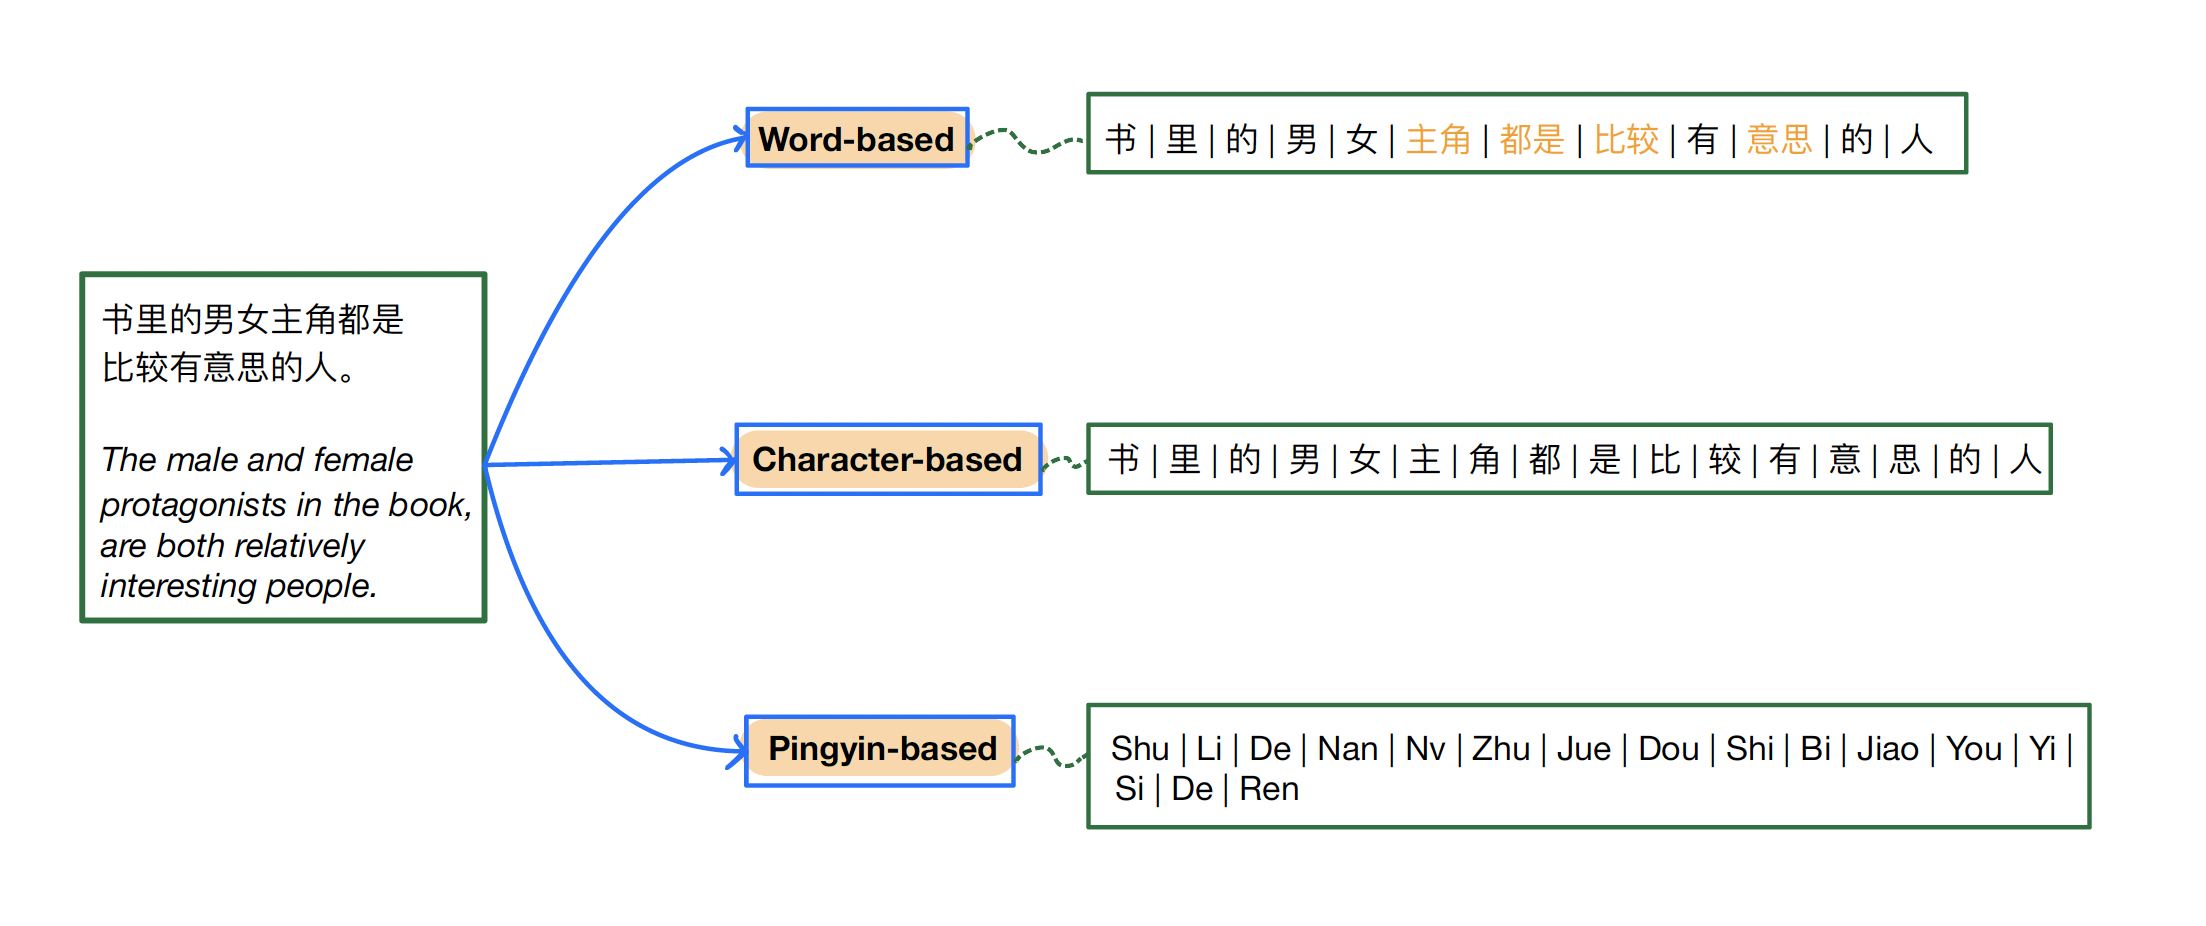
\includegraphics[width=14cm]{tokenization.png}
    \caption{Example of a sentence tokenized using different Chinese schemes: character level, word level, and pinyin level without tone.}
    \label{fig:figure1}
\end{figure*}

In this section, we describe the details of our implemented models, including LR, LSTM, BiLSTM, and a BiLSTM variant augmented with an attention layer. We also outline the dataset used for our experiments and provide details of applied data preprocessing methods.

\subsection{Logistic Regression}
The first model we implemented is LR, a statistical method designed for classification. This model predicts the likelihood of an input belonging to a certain category, using the logistic function for binary classification and the softmax function for multi-class scenarios. In our implementation, character-level tokenization was conducted straightforwardly, word-level tokenization was performed using \textit{Jieba}, and pinyin-level tokenization was carried out with the \textit{pinyin} package. The pinyin-level tokens employed do not contain tone information. For bigram feature extraction at the character level, we created bigrams directly from the character-level tokens. The features for the LR model is based on a bag-of-words approach, implemented using CountVectorizer from the \textit{sklearn} library. We trained the model with cross-entropy loss and implemented an early stopping mechanism that halts the training process if the validation loss doesn't improve for five successive epochs. The early stopping mechanism is crucial as it helps to avoid the model from overfitting to the training set. Additionally, we investigated the effect of removing Chinese stopwords, with results detailed in the Result section. 

\begin{table*}[ht]
\centering
\begin{tabular}{l l c c c c}
\hline
\textbf{Model} & \textbf{Tokenization} & \textbf{Stopword Removal} & \textbf{Vocab Size} & \textbf{Accuracy} & \textbf{F1 Score} \\ 
\hline
\hline
LR & Character & No & 4,694 & 90.30\% & 90.30\% \\
LR & Character-Bigram & No & 267,105 & \textbf{93.08\%} & \textbf{92.69\%} \\
LR & Word & No & 67,210 & 92.32\% & 92.34\% \\
LR & Pinyin & No & 501 & 85.19\% & 85.09\% \\
\hline
\hline
BiLSTM & \multirow{2}{*}{Character} & No & 4,884 & 91.85\% & 91.87\% \\
BiLSTM-w2v &  & No & 4,884 & 91.04\% & 91.20\% \\
\hline
BiLSTM & \multirow{2}{*}{Character-Bigram} & No & 304,936 & 90.57\% & 90.65\% \\
BiLSTM-w2v & & No & 304,936 & 90.42\% & 90.60\% \\
\hline
BiLSTM & \multirow{2}{*}{Word} & No & 68,495 & 90.80\% & 90.93\% \\
BiLSTM-w2v & & No & 68,495 & \textbf{92.02\%} & \textbf{91.73\%} \\
\hline
BiLSTM & Pinyin & No & 691 & 91.15\% & 91.18\% \\
\hline
\end{tabular}
\caption{Performance Comparison of LR and BiLSTM Models Using Four Tokenization Methods and Stopword Settings on \textit{onlineShopping10cats} Dataset for Sentiment Analysis}
\label{table:model_performance_sentiment}
\end{table*}


\subsection{LSTM and its variants}
We also implemented an LSTM model, tailored to address the challenges of long-range dependencies and contextual data interpretation, which is pivotal for text classification and sentiment analysis tasks~\citep{sun2022word, yuan2023}. LSTM processes text in sequence, dynamically updating its input, forget, and output states to preserve important previous context, a key factor in sentiment interpretation. Our LSTM integrates an embedding layer, potentially utilizing a pre-trained word2vec embedding, to convert tokens into vectors. The pretrained word2vec embedding\footnote{https://github.com/Embedding/Chinese-Word-Vectors/tree/master} we used, sourced from the study~\citep{li2018ana}, is capable of converting both words and characters into semantically meaningful vectors. This pretrained word2vec model covers 99.6\% of the characters in our dataset and approximately 70\% of the words resulting from \textit{Jieba}'s word-level tokenization. For the pinyin-level tokenization, word2vec embeddings is unavailable. In LSTM models that do not utilize the pretrained word2vec embedding, input tokens are initialized with random embeddings. The effectiveness of incorporating the word2vec embedding is examined in the Results section. Moreover, we evaluated the need for a bidirectional layer using the validation set. We refer to the bidirectional LSTM as BiLSTM, which is capable of capturing temporal dependencies in both forward and backward directions. The model finally utilizes a fully connected layer that assigns outputs from the LSTM layer into predefined categories. This design is effective in handling sequences of varying length.

Furthermore, we enhanced our BiLSTM model by incorporating an attention mechanism, referred to as BiLSTM\_A. The attention mechanism calculates attention scores using the outputs of hidden states from the LSTM layer, with a tanh activation and a linear projection. These scores are then used to weight the LSTM's outputs, creating a context vector that is then passed through the final layer to produce the ultimate classification results.

We employed the same tokenization schemes and bigram feature extraction methods for LSTM-based models same as we did for the LR model. In the training process, we applied the early stopping mechanism with a patience of five epochs and investigated the impact of stopwords removal for all LSTM models as well. Cross-entropy loss was utilized for training. We fine-tuned the hyper-parameters on the validation set, including the number of layers and the decision to use a bidirectional LSTM layer. Based on the model's performance with word-level tokenization, we selected two layers and a bidirectional structure. The embedding dimension was set to 300, in line with the pretrained word2vec embedding size. The final configuration for both BiLSTM and BiLSTM\_A models includes 128 hidden units, a dropout rate of 0.2, a learning rate of 0.003, and a batch size of 256.


\subsection{Dataset}
We conducted experiments on the \textit{onlineshopping10cats} dataset\footnote{https://github.com/SophonPlus/ChineseNlpCorpus/tree/master}, sourced from the ChineseNlpCorpus and uploaded in 2018. This dataset originates from user evaluations on an e-commerce website, and it contains 10 categories, including books, tablets, mobile phones, fruits, and more. This dataset comprises over 60,000 comments, equally balanced between positive and negative reviews and the 10 categories.

For data preprocessing, we first cleaned the data by removing punctuation marks and special symbols from the text. Optionally, we perform the removal of common Chinese stopwords, which are high-frequency words that do not contribute significantly to the meaning of the text. The stopwords are obtained from a GitHub repository\footnote{https://github.com/stopwords-iso/stopwords-zh}. For the purposes of model training and evaluation, the dataset was then divided: 70\% was used for training, 15\% for validation and model selection, and the remaining 15\% served as the test set. 




\section{Results}
% In this section, we present experimental results of LR and LSTM models for sentiment analysis and text classification, conducted on the onlineshopping10cats dataset.

We present the accuracy and F1 scores for LR and LSTM models under the tokenization schemes of character, character-bigram, word and pinyin in Table~\ref{table:model_performance_sentiment} and ~\ref{table:model_performance_text}. Additionally, we examine the effects of stopword removal and the incorporation of pretrained word2vec embeddings on the models' performance across these tokenization schemes. The full results, encompassing a parametric analysis of models' hyperparameters, are included in \emph{results.xlsx}, which can be found in our GitHub repository. Due to page limitation, we provide only the best results for stopword removal, one for each pair of model and tokenization scheme. The results for Bi-LSTM\_A are omitted as well as they are similar to those of the standard BiLSTM. Our source code is available in our GitHub repository\footnote{https://github.com/jyiwei/COMP550\_Course\_Project}.


\begin{table*}[ht]
\centering
\begin{tabular}{l l c c c c}
\hline
\textbf{Model} & \textbf{Tokenization} & \textbf{Stopword Removal} & \textbf{Vocab Size} & \textbf{Accuracy} & \textbf{F1 Score} \\ 
\hline
\hline
LR & Character & No & 4,694 & 88.10\% & 88.22\% \\
LR & Character-Bigram & No & 267,105 & \textbf{89.44\%} & \textbf{89.55\%} \\
LR & Word & No & 67,210 & 89.38\% & 89.50\% \\
LR & Pinyin & No & 501 & 80.58\% & 81.08\% \\
\hline
\hline
BiLSTM & \multirow{2}{*}{Character} & Yes & 4,863 & 87.36\% & 87.60\% \\
BiLSTM-w2v &  & Yes & 4,863 & 87.04\% & 87.02\% \\
\hline
BiLSTM & \multirow{2}{*}{Character-Bigram} & No & 304,936 & 83.05\% & 82.73\% \\
BiLSTM-w2v & & No & 304,936 & 82.16\% & 82.08\% \\
\hline
BiLSTM & \multirow{2}{*}{Word} & Yes & 67,869 & 85.45\% & 85.60\% \\
BiLSTM-w2v & & No & 68,495 & \textbf{87.60\%} & \textbf{87.71\%} \\
\hline
BiLSTM & Pinyin & Yes & 677 & 84.45\% & 84.68\% \\
\hline
\end{tabular}
\caption{Performance Comparison of LR and BiLSTM Models Using Various Tokenization Methods and Stopword Settings on \textit{OnlineShopping10cats} Dataset for Text Classification}
\label{table:model_performance_text}
\end{table*}


% \begin{table*}[ht]
% \centering
% \begin{tabular}{c c c c c c}
% \hline
% \textbf{Model}&\textbf{Tokenization}&\textbf{Stopwords Removal}&\textbf{Vocab Size}&\textbf{Accuracy} &\textbf{F1} \\ \hline
% LR & character & No & 4694 & 88.1 & 88.22  \\ 
% \hline
% LR & character-bigram & No & 267105 & 89.44 & 89.55 \\ \hline
% LR & word & No & 67210 & 89.38 & 89.50 \\ 
% \hline
% LR & pinyin & No & 501 & 80.58 & 81.08\\ 
% \hline
% BiLSTM & character & Yes & 4863 & 87.36 & 87.60 \\ 
% BiLSTM-w2v & character & Yes & 4863 & 87.04 & 87.02  \\ 
% \hline
% BiLSTM & character-bigram & No & 304936 & 83.05 & 82.73 \\
% BiLSTM-w2v & character-bigram & No & 304936 & 82.16 & 82.08\\ 
% \hline
% BiLSTM & word & Yes & 67869 & 85.45 & 85.60 \\ 
% BiLSTM-w2v & word & No & 68495 & 87.60 & 87.71 \\ 
% \hline
% BiLSTM & pinyin & Yes & 677 & 84.45 & 84.68 \\ 
% \hline
% \end{tabular}
% \caption{Best-Performing Accuracy and F1 of LR, BiLSTM, and BiLSTM\_A models across different tokenization schemes, stopword removal Settings, and the incorporation of pretrained word2vec embeddings on the Onlineshopping10cats dataset for text classification}
% \label{table:model_performance_sentiment}
% \end{table*}

% \begin{table*}[ht]
% \centering
% \begin{tabular}{c c c c c c}
% \hline
% \textbf{Model}&\textbf{Tokenization}&\textbf{Stopwords Removal}&\textbf{Vocab Size}&\textbf{Accuracy} &\textbf{F1} \\ \hline
% LR & character & No & 4694 & 88.1 & 88.22  \\ 
% \hline
% LR & character-bigram & No & 267105 & 89.44 & 89.55 \\ \hline
% LR & word & No & 67210 & 89.38 & 89.50 \\ 
% \hline
% LR & pinyin & No & 501 & 80.58 & 81.08\\ 
% \hline
% BiLSTM & character & Yes & 4863 & 87.36 & 87.60 \\ 
% BiLSTM-w2v & character & Yes & 4863 & 87.04 & 87.02  \\ 
% \hline
% BiLSTM & character-bigram & No & 304936 & 83.05 & 82.73 \\
% BiLSTM-w2v & character-bigram & No & 304936 & 82.16 & 82.08\\ 
% \hline
% BiLSTM & word & Yes & 67869 & 85.45 & 85.60 \\ 
% BiLSTM-w2v & word & No & 68495 & 87.60 & 87.71 \\ 
% \hline
% BiLSTM & pinyin & Yes & 677 & 84.45 & 84.68 \\ 
% \hline
% \end{tabular}
% \caption{Best-Performing Accuracy and F1 of LR, BiLSTM, and BiLSTM\_A models across different tokenization schemes, stopword removal Settings, and the incorporation of pretrained word2vec embeddings on the Onlineshopping10cats dataset for text classification}
% \label{table:model_performance_sentiment}
% \end{table*}

\subsection{Sentiment Analysis}

We observe that the results are comparable across all tokenization schemes for sentiment analysis. For the LR model with bag-of-words features, the model performs better with low-granular features such as word and character-bigram compared to features constructed from character and pinyin. In contrast, for neural models trained with distributed representations, the performance is robust to different tokenization schemes with the LSTM trained on character-level features slightly outperforming the ones fed with other features without pretrained word embeddings. When initialized with word2vec embeddings, the character-level LSTM model shows no improvements, while the word-level LSTM model exhibits a slight enhancement in performance.

The worst performing model is LR trained on toneless pinyin features with more than 5\% drop in accuracy and F1 score compared to other tokenization schemes. The large drop in performance for pinyin features is not observed in neural network models.

\subsection{Text Classification}
The results for text classification is highly similar to those of sentiment analysis with analogous patterns. The LR model performs optimally under low-granular features and only exhibits a large performance drop when trained with pinyin features. In comparison, the performance of LSTM trained with character features is the highest without word2vec embeddings. Equipped with word2vec, the performance of word-level LSTM is comparable to character-level LSTM. Specifically for text classification, character-bigram features result in a large performance drop for LSTM.  

\section{Discussion and Conclusion}

Our results indicate that, specifically for tasks defined on the chosen dataset, character-level and word-level features are equally sufficient. For neural network models, word-level features are slightly advantageous due to the availability of pretrained embeddings with rich semantics. We observe that while pretrained w2v-embeddings for Chinese words improve model performance, those for characters lead to a slight performance drop. We hypothesize that this is due to the fact that semantics encoded in individual Chinese characters are more ambiguous compared to whole words, as the meanings of constituent characters within a word can significantly differ from overall semantics of the word itself.

For LR trained with bag-of-word features, word and character-bigram are optimal. In general, these low-granular features induce sparsity in the transformed high-dimensional features space resulting in linearly separable clusters for each class.  

Surprisingly, despite the low resolution of toneless-pinyin, with less than 1000 unique tokens, models can obtain adequate results with less than 10\% difference in performance compared to the best performing model. This shows that text classification and sentiment analysis do not rely on fine semantics on our dataset.  

\subsection{Limitation and Future Work}
The main limitation of our study is its restriction to a single dataset. The tasks on this dataset might not be adequately challenging for the purpose of our investigation. As LR results in Table \ref{table:model_performance_sentiment} and \ref{table:model_performance_text} indicate, the classes for each task are linearly separable. Furthering our study on other datasets is crucial since we hypothesize that models' performance based on different feature granularity is task and dataset dependent. Another limitation is that the pretrained word2vec model we utilized covers only about 70\% of the word-level tokens. We intend to explore additional pretrained word2vec models to enhance our word and character features. 

% Additionally, we did not address the running time associated with different tokenization schemes. This aspect is crucial, especially when applying these methods to much larger datasets, due to the significant computational costs involved.


\section{Statement of Contribution}
All members contributed to the project's design. Zihan Wang coded the BiLSTM\_A model and code frame, selected the initial pre-trained word2vec model, drew figures, and proofread the report. Jack Wei coded LR and LSTM models, fixed bugs, coded for running experiments, ran experiments, and wrote results and discussion sections. Xijuan Sun found the final pre-trained word2vec model, adapted the LSTM model for it, ran experiments, and wrote the first four sections of the report.





% Entries for the entire Anthology, followed by custom entries
\bibliography{anthology,custom}
\bibliographystyle{acl_natbib}


\end{document}
